	\begin{frame}
	\myheading{Module 8.4 : $l_2$ regularization}
\end{frame}

\begin{frame}
	\vspace{4em}
	\begin{overlayarea}{\textwidth}{\textheight}
		\begin{block}{Different forms of regularization}
			\begin{itemize}
				\item \textcolor{red}{$l_2$ regularization}
				\item Dataset augmentation
				\item Parameter Sharing and tying
				\item Adding Noise to the inputs 
				\item Adding Noise to the outputs
				\item Early stopping
				\item Ensemble methods
				\item Dropout
			\end{itemize}
		\end{block}
	\end{overlayarea}
\end{frame}

	
%  3.2 YET TO COME
%%%%%%%%%%%%%%%%%%%%%%%%%%%%%%%%%%%%%%%%%%%%%%%%%%%%%%%%
\begin{frame}
	\begin{columns}
		\column{\textwidth}
		\vspace{2em}
		\begin{overlayarea}{\textwidth}{\textheight}
			\begin{itemize}
				\item<1-> For $l_2$ regularization we have,
				\begin{align*} 
					\widetilde{\mathscr{L}}(w) = \mathscr{L}(w) + \frac{\alpha}{2} \|w\|^2
				\end{align*}
				\item<2-> For SGD (or its variants), we are interested in
				\begin{align*}
					\nabla \widetilde{\mathscr{L}}(w) =  \nabla \mathscr{L}(w) + \alpha w
				\end{align*}
				\item<3-> Update rule:
				\begin{align*}
				w_{t+1} = w_t - \eta \nabla \mathscr{L}(w_t) - \eta \alpha w_t
				\end{align*}
				\item<4-> Requires a very small modification to the code
									
				\item<5-> Let us see the geometric interpretation of this
			\end{itemize}
		\end{overlayarea}
	\end{columns}
\end{frame}
	
\begin{frame}
	\begin{columns}
		\column{\textwidth}
		\begin{overlayarea}{\textwidth}{\textheight}
			\begin{itemize}
				\item<1-> Assume $w^*$ is the optimal solution for $\mathscr{L}(w)$ [not $\widetilde{\mathscr{L}}(w)$] i.e. the solution in the absence of regularization $(w^* \text{ optimal }\rightarrow \nabla \mathscr{L}(w^*) = 0)$
				\item<2-> Consider $u = w-w^{*}$. Using Taylor series approximation (upto $2^{nd}$ order)
				\begin{align*}
					\onslide<3->{\mathscr{L}(w^{*}+u)                       & = \mathscr{L}(w^{*}) + u^T \nabla \mathscr{L}(w^{*}) + \frac{1}{2} u^{T} Hu} \\ 
					\onslide<4->{  
					\mathscr{L}(w)                       & = \mathscr{L}(w^*) + (w - w^*)^T \nabla \mathscr{L}(w^*) + \frac{1}{2} (w - w^*)^T H(w - w^*) \\ }
					\onslide<5->{              & = \mathscr{L}(w^*) + \frac{1}{2} (w - w^*)^T H(w - w^*)                             
					\text{\hspace{2em} ($\because \nabla L (w^*) = 0$ )} \\}
					\onslide<6->{  \nabla \mathscr{L}(w) & = \nabla \mathscr{L}(w^*) + H(w - w^*)                                              \\}
					\onslide<7->{              & = H(w - w^*)}                                                             
				\end{align*}  
									
				\item<8-> Now,
				\begin{align*}
					\onslide<8->{\nabla \widetilde{\mathscr{L}}(w) & = \nabla \mathscr{L}(w) + \alpha w \\ }
					\onslide<9->{                        & = H(w - w^*) + \alpha w} 
				\end{align*}
									
			\end{itemize}
		\end{overlayarea}
	\end{columns}
\end{frame}
	
	
	
	
	
\begin{frame}
	\begin{columns}
		\column{\textwidth}
					
		\begin{overlayarea}{\textwidth}{\textheight}
			\vspace{2em}
			\begin{itemize}
				\item<1-> Let $\widetilde{w}$ be the optimal solution for $\widetilde{L}(w)$ [i.e regularized loss]
				\onslide<2->{
					\begin{align*}
						\because \nabla \widetilde{L}(\widetilde{w}) = 0 
					\end{align*}}
				\vspace{-1em}
				\begin{align*}
					\onslide<3->{&H(\widetilde{w} - w^*) + \alpha \widetilde{w} = 0                                      \\}
					\onslide<4->{\therefore &(H + \alpha \mathbb{I} )\widetilde{w}         = H w^*                                  \\}    
					\onslide<5->{\therefore &\widetilde{w}                                 =  (H + \alpha \mathbb{I} ) ^{-1} H w^*} 
				\end{align*}
									
				\item<6->    Notice that if $\alpha \rightarrow 0$ then $\widetilde{w} \rightarrow w^*$ [no regularization] 
				\item<7->  But we are interested in the case when $\alpha \neq 0$
				\item<8->Let us analyse the case when  $\alpha \neq 0$\hspace{-3em}
			\end{itemize}
		\end{overlayarea}
	\end{columns}
\end{frame}
	
\begin{frame}
	\begin{columns}
		\column{\textwidth}
		\begin{overlayarea}{\textwidth}{\textheight}
			\vspace{2em}
			\begin{itemize}
				\item<1-> If H is symmetric Positive Semi Definite
				\vspace{-4mm}
				\onslide<2->{\hspace{4em}\begin{align*}
					H = Q \Lambda Q^T  \text{\hspace{2em} [$Q$ is orthogonal, $QQ^T = Q^T Q = \mathbb{I}$] }  
					\end{align*}
				}
				\vspace{-1.5em}
				\begin{align*}
					\onslide<3->{\widetilde{w} & = (H + \alpha \mathbb{I})^{-1} H w^*                                       \\}
					\onslide<4->{              & = (Q \Lambda Q^T + \alpha \mathbb{I})^{-1} Q \Lambda Q^T  w^*              \\}
					\onslide<5->{              & = (Q \Lambda Q^T + \alpha Q \mathbb{I} Q^T)^{-1} Q \Lambda Q^T  w^*        \\}
					\onslide<6->{              & =  [Q( \Lambda + \alpha \mathbb{I}) Q^T ]^{-1} Q \Lambda Q^T  w^*          \\}
					\onslide<7->{              & = Q^{T^{-1}} ( \Lambda + \alpha \mathbb{I})^{-1} Q^{-1} Q \Lambda Q^T  w^* \\}
					\onslide<8->{              & = Q (\Lambda +\alpha \mathbb{I})^{-1} \Lambda Q^T w^*                      
					\text{\hspace{2em}($\because  Q^{T^{-1}} = Q$)} \\}
					\onslide<9->{\widetilde{w} & = Q D Q^T w^* }
				\end{align*} 
									
									
				\onslide<10->{where $D =  ( \Lambda + \alpha \mathbb{I})^{-1} \Lambda$, is a diagonal matrix which we will see in more detail soon}
			\end{itemize}
		\end{overlayarea}
	\end{columns}
\end{frame}
	
	
\begin{frame}   
	\begin{columns}
		\column{0.5\textwidth}
		\begin{overlayarea}{\textwidth}{\textheight}
							
			\begin{align*}
				\widetilde{w} &= Q(\Lambda + \alpha\mathbb{I})^{-1}\Lambda Q^T w^*  \\
				&= Q D Q^T w^* \\
				\onslide<5->{( \Lambda + \alpha \mathbb{I})^{-1} & = 
				\begin{bmatrix}
				\onslide<6->{\frac{1}{\lambda_1 +  \alpha}          &                                         &        &                                          \\}
				\onslide<7->{                                         & \frac{1}{\lambda_2 +  \alpha}         &        &                                          \\}
				\onslide<8->{                                         &                                         & \ddots &                                          \\}
				\onslide<9->{                                         &                                         &        & \frac{1}{\lambda_n +  \alpha}}         
				\end{bmatrix}\\}
				\onslide<10->{D &= ( \Lambda + \alpha \mathbb{I})^{-1} \Lambda\\}
				\onslide<11->{( \Lambda + \alpha \mathbb{I})^{-1} \Lambda & = 
				\begin{bmatrix}
				\onslide<12->{\frac{\lambda_1}{\lambda_1 +  \alpha} &                                         &        &                                          \\}
				\onslide<13->{                                        & \frac{\lambda_2}{\lambda_2 +  \alpha} &        &                                          \\}
				\onslide<14->{                                        &                                         & \ddots &                                          \\}
				\onslide<15->{                                        &                                         &        & \frac{\lambda_n}{\lambda_n +  \alpha}} 
				\end{bmatrix}}  
			\end{align*}
		\end{overlayarea}
					
		\column{0.5\textwidth}<1->
		\vspace{3em}
		\begin{overlayarea}{\textwidth}{\textheight}
			\begin{itemize}
				\item <1-> So what is happening here?
				\item <2->  $w^*$ first gets rotated by $Q^T$ to give $Q^Tw^*$
				\item <3->  However if $\alpha = 0$ then $Q$ rotates $Q^Tw^*$ back to give $w^*$
				\item <4->  If $\alpha \neq 0$ then let us see what $D$ looks like
				\item <16->  So what is happening now?
			\end{itemize}
		\end{overlayarea}
	\end{columns}
\end{frame}
	
\begin{frame}
	\begin{columns}
		\column{0.5\textwidth}
		\begin{overlayarea}{\textwidth}{\textheight}
			\begin{align*}
				\widetilde{w} &= Q(\Lambda + \alpha\mathbb{I})^{-1}\Lambda Q^T w^*  \\
				&= Q D Q^T w^* \\
				\onslide<1->{( \Lambda + \alpha \mathbb{I})^{-1} & = 
				\begin{bmatrix}
				\onslide<1->{\frac{1}{\lambda_1 +  \alpha}         &                                         &        &                                          \\}
				\onslide<1->{                                        & \frac{1}{\lambda_2 +  \alpha}         &        &                                          \\}
				\onslide<1->{                                        &                                         & \ddots &                                          \\}
				\onslide<1->{                                        &                                         &        & \frac{1}{\lambda_n +  \alpha}}         
				\end{bmatrix}\\}
				\onslide<1->{D &= ( \Lambda + \alpha \mathbb{I})^{-1} \Lambda\\}
				\onslide<1->{( \Lambda + \alpha \mathbb{I})^{-1} \Lambda & = 
				\begin{bmatrix}
				\onslide<1->{\frac{\lambda_1}{\lambda_1 +  \alpha} &                                         &        &                                          \\}
				\onslide<1->{                                        & \frac{\lambda_2}{\lambda_2 +  \alpha} &        &                                          \\}
				\onslide<1->{                                        &                                         & \ddots &                                          \\}
				\onslide<1->{                                        &                                         &        & \frac{\lambda_n}{\lambda_n +  \alpha}} 
				\end{bmatrix}}  
			\end{align*}
		\end{overlayarea}
					
		\column{0.5\textwidth}<1->
		\vspace{3em}
		\begin{overlayarea}{\textwidth}{\textheight}
			%T\begin{block}<1->{}
			\begin{itemize}
				\item <1->  Each element $i$ of $Q^T w^*$ gets scaled by $\frac{\lambda_i}{\lambda_i + \alpha} $ before it is rotated back by $Q$
				\item <2->  if $\lambda_i >> \alpha$ then $\frac{\lambda_i}{\lambda_i + \alpha} = 1$
				\item <3->  if $\lambda_i << \alpha$ then $\frac{\lambda_i}{\lambda_i + \alpha} = 0$
				\item <4->  Thus only significant directions (larger eigen values) will  be retained.  
				\begin{align*}
					\text{Effective parameters} = \sum_{i=1}^{n} \frac{\lambda_i}{\lambda_i+\alpha} < n
				\end{align*}
			\end{itemize}
		\end{overlayarea}
	\end{columns}
\end{frame}

\begin{frame}
			
	\begin{figure}
		\centering
		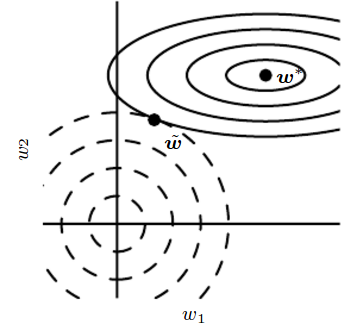
\includegraphics[width=0.35\linewidth]{./images/7_1DL}
		\caption*{}
		\label{fig:7_1DL}
	\end{figure}
	
	\begin{itemize}
		\item<2-> The weight vector($w^*$) is getting rotated to ($\tilde{w}$)
		\item<3-> All of its elements are shrinking but some are shrinking more than the others
		\item<4-> This ensures that only important features are given high weights
	\end{itemize}
\end{frame}
